\documentclass[12pt]{article}
\usepackage{mathptmx}
\usepackage[margin=1in]{geometry}
\usepackage{amsmath,amssymb,amsthm,graphicx}
\newtheorem{proposition}{Proposition}
\newtheorem{theorem}{Theorem}
\newtheorem{lemma}{Lemma}
\newtheorem{definition}{Definition}
\newtheorem{remark}{Remark}

% ---- result macros (filled from study outputs) ----
\newcommand{\Npos}{24{,}628}
\newcommand{\Nneg}{24{,}628}
\newcommand{\Nclusters}{12{,}110}
\newcommand{\Ntrain}{40{,}776}
\newcommand{\Nval}{4{,}094}
\newcommand{\Ntest}{4{,}386}

\title{Antimicrobial Peptide Design and Discovery with Convolutional and
Graph Neural Networks: Homology-Aware Benchmarks, External Validation on
APD6, and a Discovery Screen over Uncharacterized Proteins}
\author{MEGA-Program-27, Item 9 Part 1 (lane 09a)}
\date{September 24, 2026}

\begin{document}
\maketitle

\begin{abstract}
Antimicrobial peptides (AMPs) are a structurally diverse class of host-defense
molecules and a candidate answer to antibiotic resistance. We study AMP
recognition and design with two neural architectures --- a convolutional
network (PepCNN) over a joint one-hot/physicochemical sequence encoding and a
graph neural network (PepGNN) over a residue graph with a shared positional
adjacency --- trained and evaluated on 24{,}628 reviewed UniProt
KW-0929 AMPs against 24{,}628 length-matched non-AMP proteins, with
cluster-aware train/validation/test splits that prevent homology leakage.
PepCNN attains AUROC $0.947$ [0.936, 0.955] under 5-fold cross-validation on a
curated 2{,}732-sequence pilot and $0.921$ [0.913, 0.929] on the held-out
large-scale test split; a random-forest baseline on dipeptide composition is
competitive on the pilot (0.935) but the convolutional model dominates at
scale and on external validation against the APD6 2024 natural AMP list.
We prove fixed-temperature detailed balance of a simulated-annealing
transition used to propose untested candidate sequences, derive the permutation and bootstrap procedures
used for significance, and report an in-silico discovery screen over 852
reviewed uncharacterized proteins of 10--60 residues. On the published AMP Scanner Vr.2 benchmark our stacked ensemble is near
the original model on its own test partition but below the later ACEP model.
We additionally audit an updated Feb2020 production dataset with 10-fold
cross-validation; comparability limits and detailed results are reported. Eight screened proteins and one annealed design are named as testable
candidates with quantified pairwise 3-mer similarity checks against APD6 and
a UniProt KW-0929 subsample, not established antimicrobial discoveries. All results are
reproducible from the accompanying repository; claims are limited to what the
data support.
\end{abstract}

\section{Introduction}
The spread of antibiotic resistance has renewed interest in antimicrobial
peptides (AMPs), short cationic and often amphipathic sequences that disrupt
microbial membranes and are harder for bacteria to evade than small-molecule
antibiotics~\cite{apd3,wang2016}. Databases such as the APD (now
APD6)~\cite{apd3} and DBAASP~\cite{dbaasp} curate thousands of experimentally
characterized AMPs, and UniProt keyword KW-0929 annotates reviewed
antimicrobial proteins at scale~\cite{uniprot}. Computational screening and
design of AMPs is attractive because the sequence space is enormous: even at
length 25 there are $20^{25} \approx 3.4\times 10^{32}$ candidates, of which
only a minuscule fraction has been assayed.

This paper, item 9 part 1 of the MEGA-Program-27 series, asks three questions.
(1) How well do convolutional and graph neural networks recognize AMPs when
evaluation is protected against homology leakage --- the dominant confound in
peptide classification benchmarks? (2) Do models trained on UniProt KW-0929
generalize to an independently curated resource, APD6? (3) Can the trained
models prioritize plausible novel AMPs, both by free design (simulated
annealing against the learned score) and by screening uncharacterized
proteins?

\subsection{Biological setting}
AMPs are produced across all domains of life. The canonical family --- short,
net-cationic, amphipathic peptides such as magainins, LL-37, and the
defensins --- partitions into microbial membranes and kills by
permeabilization, but the known universe also includes anionic AMPs,
glycine-rich peptides, proline-rich peptides that enter cells and inhibit
translation, and larger disulfide-stabilized folds. This mechanistic variety
is the central recognition challenge: there is no single sequence signature,
and any single-feature rule (charge, hydrophobic moment, length) fails on
whole families. It is also why we treat sensitivity numbers honestly: a model
trained on a corpus dominated by short cationic peptides should not be
expected to score disulfide-locked anionic families highly, but per-family sensitivity has not yet been measured in this study.

\subsection{Contributions}
\begin{enumerate}
\item An auditable, exact-10-mer cluster-split benchmark with a subsequently
identified source-review confound:
24{,}628 UniProt KW-0929 positives (mostly unreviewed) against 24{,}628 length-matched
reviewed negatives, clustered by shared exact 10-mers into 12{,}110
components and split 80/10/10 by cluster, with all fetch URLs, hashes, and
timestamps recorded.
\item A paired comparison of two neural architectures and two composition
baselines under this split, with bootstrap intervals and permutation tests
computed by one shared harness: PepCNN attains descriptive AUROC $0.921$ [0.913, 0.929] on the confounded
held-out sample, ahead of the tested baselines; the graph model is a reported negative
result.
\item An APD6 2024 positive-versus-reviewed-UniProt-negative comparison after exact-10-mer filtering:
PepCNN scores AUROC $0.926$ [0.918, 0.934] and sensitivity $0.601$ at a
5\% false-positive rate, but review-status confounding in training limits
its biological interpretation.
\item A simulated-annealing designer with a fixed-temperature detailed-balance
proof producing ranked sequence candidates, and a discovery
screen over 852 reviewed uncharacterized proteins producing 25 ranked
hypotheses, all clearly labeled as in-silico.
\item A reproducible software artifact: the \texttt{pepdesign} package, multiple study scripts, a 27-test hermetic suite, and reproducible
benchmark and candidate tables derived from checked-in result files.
\end{enumerate}

\subsection{Scope}
This paper is bounded to an AMP benchmark provenance audit and its exploratory recognition, design and screening work. No activity against specific strains, toxicity, structural mechanism or wet-lab outcome is inferred from binary labels and unassayed sequences.

\subsection{Notation and organization}
\begin{table}[h]\centering\caption{Notation used throughout.}
\begin{tabular}{ll}\hline
Symbol & Meaning \\ \hline
$s$, $\ell$ & a peptide sequence and its length \\
$L$ & encoding cap (150; pilot 60; full Feb2020 audit 200) \\
$K_k(s)$ & set of contiguous $k$-mers of $s$ \\
$E(s)$ & encoded sequence, $\mathbb{R}^{L\times(20+d)}$ \\
$\tilde A$ & symmetric-normalized shared adjacency \\
$\hat p$, $f(s)$ & sigmoid classifier output and ensemble score \\
$\omega$ & positive-class weight $n_-/n_+$ \\
$\pi_T(s)$, $T$ & fixed-temperature Boltzmann measure and temperature \\
$J(\cdot,\cdot)$ & Jaccard index \\
$B$ & resampling count (bootstrap or permutation) \\
\hline\end{tabular}\end{table}

Section 2 situates the work; Section 3 defines the data, clustering, and
splits; Section 4 defines the models, objective, designer, and statistical
procedures, with proofs; Section 5 fixes the evaluation metrics; Later sections report the benchmark studies, candidate screen, signal
ablation, threats, reproducibility audit and software artifact. Appendices
give hyperparameters, provenance and design/screen listings.

\section{Related Work}
The APD has been curated since 2003; its third version, APD3, organized AMP
annotation and search~\cite{apd3}, and the 2024 APD6 release provides
downloadable FASTA lists of natural AMPs with known activity. DBAASP adds
experimentally measured activities and targets~\cite{dbaasp}. Machine-learning
AMP classifiers span support-vector machines and random forests on
composition features (e.g., CAMP~\cite{camp}) to recurrent and convolutional
architectures such as AMPScanner~\cite{ampscanner}. Most published benchmarks
split sequences randomly, which leaks near-duplicates across train and test;
we instead cluster on shared $k$-mers and split clusters. Our graph model is
related to message-passing networks~\cite{gilmer2017} with a fixed
chain-adjacency structure rather than a learned or contact-derived graph.

\subsection{AMP databases}
The APD has tracked the natural AMP literature since 2003; the APD3
release~\cite{apd3} introduced a unified search and annotation interface, and
the current APD6 site distributes curated FASTA lists, including the 2024
natural-AMP list (3{,}306 entries) used here as external validation. DBAASP
takes a different angle: it curates peptides together with experimentally
measured activities against specific strains, making it the richer resource
for potency modeling but a harder one to mirror programmatically; during this
work its full-dataset endpoint returned empty responses to non-interactive
requests, so we cite it but do not benchmark against it
(Section 8). CAMP~\cite{camp} and its associated predictors remain widely
used baselines; DRAMP and LAMP aggregate overlapping records. These resources
differ in curation policy, redundancy, and label semantics, which is exactly
why cross-database evaluation --- training on UniProt KW-0929 and testing on
APD6 --- is more informative than a second random split of the same source.

\subsection{Machine-learning AMP recognition}
Early predictors used composition features with classical models: CAMP's
built-in SVM and random-forest classifiers~\cite{camp} and a long tail of
composition-plus-SVM tools. Deep approaches followed: AMPScanner applied
recurrent and convolutional networks to raw sequences~\cite{ampscanner}, and
subsequent work explored attention and pretrained protein language models.
Two methodological concerns recur across this literature. First, most
evaluations split sequences randomly, and AMP families are highly redundant
--- many database records are isoforms or orthologs --- which can inflate random-split metrics; a high AUROC alone does not
quantify memorization without a homology-aware control.
Second, negative sets are usually ``everything else,'' which conflates
unlabeled positives with true negatives. Our design choices respond directly:
cluster-aware splitting controls the first, length-matched reviewed negatives
acknowledge the second (without eliminating it), and external validation on
an independently curated database tests whether the learned function is
about AMPs or about the training corpus.

\subsection{AMP design}
Computational AMP design has used genetic algorithms, physicochemical rules,
and generative models including GANs, VAEs, and diffusion-style generators.
A common weakness is evaluation: generated sequences are often scored by the
same model that guided generation, an echo chamber that inflates apparent
quality. We keep the designer simple: simulated annealing on a discriminative
ensemble, with a proof of fixed-temperature detailed balance and an
explicit pairwise 3-mer similarity check against the reference corpus.
That check does not prove global novelty, and optimization on the scoring
model cannot independently validate its own designs. No design is claimed active; the section exists to
demonstrate a correct, reproducible prioritization mechanism.

\section{Data}
\subsection{Positive set}
All reviewed UniProtKB entries carrying keyword KW-0929 (antimicrobial) with
sequence length 10--150 were streamed from the UniProt REST API on
September 24, 2026 (27{,}392 records). After restricting to the 20 standard
amino acids and de-duplicating, \Npos{} positives remained.

\subsection{Negative pool and length matching}
A pool of 105{,}041 reviewed entries of length 10--150 \emph{without} KW-0929
was streamed under identical conditions. Negatives were sampled to match the
positive length distribution, yielding \Nneg{} negatives.

\subsection{Homology-aware clustering and splits}
Random splits of peptide corpora leak homologs: a sequence differing from a
training sequence by a few residues may appear in test, inflating metrics.
We cluster with union-find over shared exact 10-mers
(Definition~\ref{def:cluster}), producing \Nclusters{} clusters, then assign
whole clusters to train/validation/test in proportions 80/10/10
(\Ntrain{}/\Nval{}/\Ntest{} sequences).

\begin{definition}[$k$-mer connected clustering]\label{def:cluster}
Let $K(s)$ be the set of contiguous $k$-mers of sequence $s$. Define a graph
on sequences with edge $(s,t)$ iff $K(s)\cap K(t)\neq\emptyset$. Clusters are
its connected components, computed with union-find in
$O(\sum_s |K(s)|\,\alpha(n))$ time, where $\alpha$ is the inverse Ackermann
function.
\end{definition}

\begin{remark}
Shared exact 10-mers are a strict leakage criterion for length-10--150
peptides: two sequences sharing an exact decamer are merged; aligned homologs with
no exact decamer can still cross the split. It can also merge unrelated sequences with a low-complexity decamer,
reducing the number of independent split units.
\end{remark}

\subsection{External and screen sets}
For external validation we use the APD6 2024 natural AMP list (3{,}306
entries)~\cite{apd3}, restricted to standard residues, length 10--150,
de-duplicated, and decontaminated against the training split by the same
10-mer criterion. For the discovery screen we fetched 852 reviewed UniProt
entries of length 10--60 whose protein name is ``uncharacterized'' or
``hypothetical'', excluding KW-0929.

\section{Methods}
\subsection{Sequence encoding}
Each sequence $s$ of length at most $L=150$ is encoded as
$X\in\{0,1\}^{L\times 20}$ (one-hot) concatenated channel-wise with
per-residue physicochemical features $Z\in\mathbb{R}^{L\times d}$,
$d$ covering hydrophobicity, charge, and related scales, giving
$E(s)=[X\;Z]\in\mathbb{R}^{L\times(20+d)}$. Zero-padding follows the sequence. No explicit mask is used, a potential
length and padding confound that should be tested in future work.

\subsection{PepCNN}
PepCNN applies 1-D convolutions of kernel width $k$ over the residue axis,
\[
H^{(1)} = \phi\!\left(W^{(1)} * E(s) + b^{(1)}\right),\qquad
H^{(2)} = \phi\!\left(W^{(2)} * H^{(1)} + b^{(2)}\right),
\]
with $\phi=\mathrm{ReLU}$, followed by global max pooling and a
linear readout $\hat p = \sigma(w^\top h + c)$. Multi-scale motif detectors
fall out of the learned kernels; max pooling makes the score invariant to
motif position, matching the biology of membrane-active motifs.

\subsection{PepGNN}
Each sequence is represented by four per-residue physicochemical channels
and a \emph{shared} chain-window adjacency $A$ connecting positions within
three residues plus self-loops, identical for every sample. Each of three
graph-convolution layers computes
\[
H = \phi\!\left(\tilde A X W + b\right),\qquad
\tilde A = D^{-1/2} A D^{-1/2},
\]
with the symmetric normalization of~\cite{kipf2017}. Because $\tilde A$ is
shared, the batched product is a single broadcast matrix multiplication
rather than $n$ per-sample multiplications of $L\times L$ matrices; memory
drops from $O(nL^2)$ to $O(L^2)$ for a shared adjacency, which is what makes the model
trainable within the sandbox budget.

\begin{remark}
A chain graph is a weak prior --- it cannot encode contacts between residues
distant in sequence but close in space. Section~\ref{sec:results} shows the
GNN underperforms the CNN here; we report this as a negative architectural
result rather than tuning until it wins.
\end{remark}

\subsection{Training objective}
With class imbalance $n_+/n_- = r$, we minimize the weighted binary
cross-entropy
\[
\mathcal{L} = -\frac{1}{n}\sum_{i=1}^{n}\left[
\omega\, y_i \log \hat p_i + (1-y_i)\log(1-\hat p_i)\right],
\qquad \omega = \frac{n_-}{n_+}.
\]
\begin{proposition}[Calibration of the weighted objective]
The minimizer of the population weighted BCE satisfies
$\hat p^\ast(x) = \dfrac{\omega\, p(x)}{\omega\, p(x) + (1-p(x))}$ where
$p(x)=P(y{=}1\mid x)$; it is a strictly monotone reparametrization of the
Bayes posterior, so threshold-independent ranking metrics (AUROC, AUPRC) are
unaffected by the weighting.
\end{proposition}
\begin{proof}
Pointwise in $x$, the expected loss is
$-[\omega p \log \hat p + (1-p)\log(1-\hat p)]$; setting its derivative in
$\hat p$ to zero gives $\omega p (1-\hat p) = (1-p)\hat p$, hence the claim.
Monotonicity follows from
$\partial \hat p^\ast/\partial p = \omega/(\omega p + 1 - p)^2 > 0$.
\end{proof}

\subsection{Significance and intervals}
We report two nonparametric procedures, both computed exactly as stated.
\begin{definition}[Label-permutation test]
Under $H_0$ that scores carry no label information, the AUROC of any fixed
scoring rule computed on labels permuted uniformly at random has the same
distribution as the observed AUROC. With $B$ permutations the Monte Carlo
$p$-value is $(1+\#\{b: T_b \ge T_{\text{obs}}\})/(1+B)$, which is exact for
exchangeable nulls up to Monte Carlo error~\cite{permutation}.
\end{definition}
\begin{definition}[Bootstrap confidence interval]
Resample test pairs $(y_i, s_i)$ with replacement $B$ times; the percentile
interval $[\hat\theta_{2.5},\hat\theta_{97.5}]$ of the resampled statistics
estimates uncertainty under independent sampling, but can have poor
coverage under homology clustering~\cite{efron1994}.
\end{definition}

\subsection{Annealing designer}
The implemented proposal replaces one residue by a different canonical
amino acid, and with probability 0.2 makes a second independent replacement.
Let $f(s)$ be the ensemble score in $[0,1]$ and
$\mathcal V=\{s:\nu_3(s;\mathcal R)\ge\nu_0\}$ the allowed sequences.
At a fixed positive temperature $T$, a valid current sequence, and symmetric
proposal $q$, the transition accepts a valid proposal with probability
$\alpha_T(s,s')=\min\{1,\exp[(f(s')-f(s))/T]\}$.
The actual script changes $T$ geometrically after each step and reports the
highest-scoring visited state; its finite trajectory is therefore an
optimization heuristic, not a sample from an equilibrium distribution.
\begin{proposition}[Fixed-temperature detailed balance]
For a valid initial state and fixed $T$, the restricted transition kernel is
reversible with respect to
$\pi_T(s)\propto \exp[f(s)/T]1_{\{s\in\mathcal V\}}$.
\end{proposition}
\begin{proof}
Each single mutation has a symmetric reverse with probability
$1/(19L)$; the mixture of one- and two-mutation kernels is symmetric.
Proposals outside $\mathcal V$ are rejected. For $s,s'\in\mathcal V$,
$\pi_T(s)q(s'|s)\alpha_T(s,s')$ equals
$Z^{-1}q(s'|s)\min\{e^{f(s)/T},e^{f(s')/T}\}$, symmetric in $s,s'$.
Rejection handles diagonal mass, so detailed balance holds. We do not
claim convergence of the implemented cooling schedule.
\end{proof}

\begin{remark}
A learned score is not a certificate of antimicrobial activity. Novelty is
$1-\max_{c\in\mathcal R}J_3(s,c)$, a pairwise 3-mer Jaccard distance
against the chosen reference corpus.
\end{remark}

\subsection{Encoding details}
The physicochemical channel block $Z$ replicates, at every position, a
per-residue vector of standardized scales: Kyte--Doolittle hydrophobicity,
net charge at physiological pH ($+1$ for K/R, $-1$ for D/E, $+0.1$ for H),
molecular volume, polarity, and a helix propensity index. Each scale is
min-max standardized over the 20 residues. Concatenating $Z$ with the one-hot
block lets the first convolution learn jointly over identity and property
space; ablations are out of scope for the sandbox budget but are noted as
future work.

\subsection{Graph propagation, derived}
The GNN layer of Section 4.3 can be written as a fixed two-step filter. With
$\tilde A = D^{-1/2}(A_{\text{chain}} + \lambda I)D^{-1/2}$, one application
replaces each residue's features by a degree-weighted mean of itself and its
chain neighbors, followed by a shared linear map $W$ and nonlinearity. For
the infinite chain the filter approximates, in the graph-Fourier basis, a
low-pass kernel: eigenvalues of $\tilde A$ cluster in $[0, 2)$, and powers of
$\tilde A$ contract high-frequency components at rate $(1-\mu_2)^t$ where
$\mu_2$ is the spectral gap. A single layer therefore smooths residue
features over a window of two positions --- strictly less positional context
than a width-5 convolution, which is the simplest explanation of the observed
performance gap (Tables~\ref{tab:pilot}--\ref{tab:apd}). Stacking layers
widens the smoothing window but shrinks gradients and, for a chain, cannot
recover the position-selective max-pooling that drives the CNN.

\begin{proposition}[Shared-adjacency batching is exact]
For a batch of $n$ sequences sharing $\tilde A$, broadcasting one matrix
$\tilde A$ against the stacked feature tensor $X\in\mathbb{R}^{n\times L\times F}$
computes exactly the $n$ independent products $\tilde A X_i$.
\end{proposition}
\begin{proof}
The broadcast product $Y = \tilde A X$ has entries
$Y_{bij} = \sum_k \tilde A_{ik} X_{bkj} = (\tilde A X_b)_{ij}$ by definition
of matrix multiplication along the last two axes.
\end{proof}

\subsection{Novelty metric}
The design and screen tables report
$\mathrm{novelty}(s) = 1 - \max_{c \in C} J(K_3(s), K_3(c))$ where $C$ is the
AMP training corpus and $J$ the Jaccard index over 3-mer sets. Three-mers are
short enough that even unrelated peptides share some, so novelty is bounded
away from 1 in practice; values near 0.9 indicate essentially no local
compositional overlap with any training AMP. The metric is intentionally
cheap and interpretable; alignment-based novelty would be stricter and is
listed as future work.

\subsection{Metric definitions and identities}
All recognition claims use two threshold-free metrics.
\begin{definition}[AUROC]
For scores $s_i$ and labels $y_i\in\{0,1\}$,
$\mathrm{AUROC} = P(s_i > s_j \mid y_i{=}1, y_j{=}0) + \tfrac12 P(s_i = s_j)$,
the area under the receiver operating characteristic curve traced by varying
the decision threshold.
\end{definition}
\begin{proposition}[Mann--Whitney identity]\label{prop:mw}
Let $U$ be the number of positive--negative pairs with $s_i > s_j$ plus half
the ties. Then $\mathrm{AUROC} = U/(n_+ n_-)$ exactly, and under the null of
no label information $\mathrm{AUROC}$ concentrates around $1/2$ with
variance $(n_+ + n_- + 1)/(12 n_+ n_-)$.
\end{proposition}
\begin{proof}[Proof sketch]
The ROC curve is the empirical survival function of positive scores against
that of negatives; integrating by parts turns the area into the pairwise
probability. The variance formula is the standard Mann--Whitney null variance
under exchangeability of the pooled sample.
\end{proof}
\begin{definition}[AUPRC]
With precision $\pi(t) = P(y{=}1 \mid s \ge t)$ and recall
$\rho(t) = P(s \ge t \mid y{=}1)$, $\mathrm{AUPRC} = \int_0^1 \pi\, d\rho$,
estimated by average precision.
\end{definition}
AUPRC is the more sensitive metric under class imbalance because it ignores
true negatives entirely; our test split is balanced, so the two metrics track
each other, and the observed AUPRC gaps (e.g.\ GNN $0.680$ vs CNN $0.879$ on
the scale-up test) are the more informative signal of ranking quality in the
high-score region that the design and screen stages consume.

\subsection{Operating points}
The 5\% FPR operating point used for APD6 sensitivity is chosen on the
held-out negatives only: the threshold is the 95th percentile of ensemble
scores over the 2{,}925 test negatives, then applied to the APD6 positives.
Because the threshold never touches the positive scores, the sensitivity
estimate is an honest one-sided generalization measurement rather than a
fitted operating point.

\subsection{Physicochemical descriptors: definitions and derivations}
\label{sec:physchem-math}

The discovery audit and the tree-based baseline use four classical
descriptors. We state them precisely and derive the properties we rely on.

\begin{definition}[Net charge at pH $p$]
For residue $a$ with side-chain $\mathrm{p}K_a$, the Henderson--Hasselbalch
equation gives the protonated fraction of a basic group and the
deprotonated fraction of an acidic group as
\begin{equation}
f^{+}_a(p) = \frac{10^{\mathrm{p}K_a}}{10^{p} + 10^{\mathrm{p}K_a}}
\qquad
f^{-}_a(p) = \frac{10^{p}}{10^{p} + 10^{\mathrm{p}K_a}},
\label{eq:hh}
\end{equation}
and the expected net charge of sequence $s = s_1\cdots s_n$ at pH $p$ is
\begin{equation}
Q(s; p) = f^{+}_{\mathrm{N\text{-}term}}(p)
  + \!\!\sum_{a \in \{K,R,H\}}\!\! n_a(s)\, f^{+}_a(p)
  - f^{-}_{\mathrm{C\text{-}term}}(p)
  - \!\!\sum_{a \in \{D,E,C,Y\}}\!\! n_a(s)\, f^{-}_a(p),
\label{eq:netcharge}
\end{equation}
where $n_a(s)$ counts occurrences of $a$ in $s$ and we use
$\mathrm{p}K_a$ values $K{=}10.5$, $R{=}12.4$, $H{=}6.0$, $D{=}3.9$,
$E{=}4.1$, $C{=}8.3$, $Y{=}10.1$, N-terminus $7.0$, C-terminus $2.34$.
We evaluate $Q(s) := Q(s; 7.4)$.
\end{definition}

\begin{proposition}[Monotonicity of net charge]
\label{prop:charge-monotone}
$Q(s; p)$ is strictly decreasing in $p$ for every nonempty
sequence in this model because its termini are ionizable, with $\lim_{p\to 0} Q = n_K + n_R + n_H + 1$ and
$\lim_{p\to\infty} Q = -(n_D + n_E + n_C + n_Y) - 1$.
\end{proposition}
\begin{proof}
Each term in \eqref{eq:hh} is a logistic function of $p$:
$f^{+}_a(p) = \sigma(\ln 10 \cdot (\mathrm{p}K_a - p))$ is strictly
decreasing in $p$ and $f^{-}_a(p) = \sigma(\ln 10 \cdot (p - \mathrm{p}K_a))$
strictly increasing. $Q(s;p)$ is a positive combination of the decreasing
terms minus a positive combination of the increasing terms, hence strictly decreasing because at least the terminal terms are present. The limits follow
from $\lim_{x\to-\infty}\sigma(x) = 0$ and $\lim_{x\to\infty}\sigma(x) = 1$
applied term by term.
\end{proof}

\begin{definition}[Eisenberg hydrophobic moment]
For window length $w$ and helix angle $\delta$ ($100^\circ$ for an
$\alpha$-helix), the hydrophobic moment of window $s_{i+1}\cdots s_{i+w}$
with Kyte--Doolittle hydropathy values $h_j$ is
\begin{equation}
\mu_i(s; w, \delta) = \frac{1}{w}\left[\left(\sum_{j=1}^{w} h_j \cos j\delta\right)^2
  + \left(\sum_{j=1}^{w} h_j \sin j\delta\right)^2\right]^{1/2},
\label{eq:hmoment}
\end{equation}
and $\mu_H(s) = \max_i \mu_i(s; 11, 100^\circ)$.
\end{definition}

\begin{remark}
Equation \eqref{eq:hmoment} is the length of the mean resultant vector of
the hydropathy values placed at successive residues of a regular helix; it
is maximal exactly when the hydrophobic residues cluster on one face, the
amphipathicity that membrane-active helices exploit. This is the standard
Eisenberg consensus moment.
\end{remark}

\begin{definition}[Pairwise $k$-mer novelty]
For sequence $s$, reference corpus $\mathcal R$, and set $K_k(s)$ of
contiguous $k$-mers, define
\begin{equation}
J_k(s,r)=\frac{|K_k(s)\cap K_k(r)|}{|K_k(s)\cup K_k(r)|},\qquad
\nu_k(s;\mathcal R)=1-\max_{r\in\mathcal R} J_k(s,r).
\label{eq:novelty}
\end{equation}
This is distance from the nearest individual reference under the Jaccard
metric, not the fraction of $k$-mers missing from the union of the corpus.
A high score establishes only weak local sequence similarity; it does not
establish absence from every database or imply a new biological function.
\end{definition}

\begin{proposition}[Nearest-neighbor interpretation]
If $\mathcal R$ is finite and nonempty, $0\leq\nu_k\leq1$,
and $\nu_k(s;\mathcal R)=0$ exactly when at least one reference has the same
set of $k$-mers as $s$.
\end{proposition}
\begin{proof}
$0\leq |A\cap B|\leq |A\cup B|$ for any nonempty finite sets $A,B$,
so $0\leq J_k\leq1$. A finite maximum reaches one precisely if
$K_k(s)=K_k(r)$ for some $r$. Subtracting from one proves both claims.
Notice that equal $k$-mer sets do not imply identical sequences.
\end{proof}

\subsection{Stacked generalization}
\label{sec:stack-math}

Let $b_1, \dots, b_B$ be base scorers trained on the training partition
and let $z(x) = (b_1(x), \dots, b_B(x))^\top \in [0,1]^B$ be the score
vector on the tune partition. The stacking rule is the logistic model
\begin{equation}
g(x) = \sigma(w^\top z(x) + w_0), \qquad
\hat w = \arg\min_{w} \sum_{(x,y) \in \mathcal{T}_{\mathrm{tune}}}
  \ell(y, w^\top z(x) + w_0) + \lambda \|w\|_2^2,
\label{eq:stack}
\end{equation}
with $\ell(y, u) = \log(1 + e^{u}) - yu$.

\begin{proposition}[Convexity and gradient of the stacking objective]
\label{prop:stack-convex}
The objective \eqref{eq:stack} is convex in $(w,w_0)$ and strictly convex
when the augmented tune-partition design matrix $[Z,\mathbf1]$ has full
column rank and all fitted probabilities lie strictly between zero and one, with gradient
$\nabla_w = Z^\top(\sigma(Zw + w_0\mathbf 1) - y) + 2\lambda w$.
\end{proposition}
\begin{proof}
$\ell(y, u)$ is convex in $u$ since
$\partial^2 \ell / \partial u^2 = \sigma(u)(1-\sigma(u)) \ge 0$;
composition with the affine map $(w,w_0) \mapsto w^\top z + w_0$ preserves
convexity, and $\lambda\|w\|_2^2$ adds strict convexity in $w$ for
$\lambda > 0$. Positive logistic curvature plus full rank of the
augmented design makes the Hessian positive definite. The gradient follows from
$\partial \ell / \partial u = \sigma(u) - y$ and the chain rule.
\end{proof}

\subsection{The Matthews correlation coefficient}
\label{sec:mcc-math}

\begin{proposition}[MCC is a Pearson coefficient]
\label{prop:mcc}
For nonconstant binary predictions $\hat y$ and labels $y$ with nonzero
class counts and confusion counts
$TP, TN, FP, FN$,
\begin{equation}
\mathrm{MCC} = \frac{TP \cdot TN - FP \cdot FN}
 {\sqrt{(TP{+}FP)(TP{+}FN)(TN{+}FP)(TN{+}FN)}}
 = \phi(y, \hat y),
\label{eq:mcc}
\end{equation}
the Pearson correlation of the binary vectors; equivalently
$\mathrm{MCC}^2 = \chi^2 / N$ for the $2\times 2$ contingency table.
\end{proposition}
\begin{proof}
For binary vectors, $\mathrm{cov}(y,\hat y) = \frac{TP}{N} -
\frac{(TP{+}FN)(TP{+}FP)}{N^2} = \frac{TP \cdot TN - FP \cdot FN}{N^2}$
after expanding $(TP{+}TN{+}FP{+}FN) = N$, and
$\mathrm{var}(y) = \frac{(TP{+}FN)(TN{+}FP)}{N^2}$,
$\mathrm{var}(\hat y) = \frac{(TP{+}FP)(TN{+}FN)}{N^2}$. Substitution into
$\phi = \mathrm{cov}/\sqrt{\mathrm{var}(y)\mathrm{var}(\hat y)}$ gives
\eqref{eq:mcc}; the $\chi^2$ identity is the standard
$\chi^2 = N\phi^2$ for $2 \times 2$ tables.
\end{proof}

Unlike accuracy, MCC reflects all four confusion-matrix cells; it is
undefined mathematically when a prediction or label vector is constant,
though some software conventions return zero. We report the specified
software implementation for each benchmark comparison.

\section{Experiments}\label{sec:results}
% STUDY07/08/09 RESULT TABLES GO HERE
\subsection{Pilot study (study01)}
The pilot used the curated handoff corpus: 1{,}232 AMP-labeled peptide sequences with synthetic FASTA
identifiers and unverified source provenance (8--60 aa) and 1{,}500 length-matched non-AMP negatives, evaluated
by 5-fold cross-validation with bootstrap intervals ($B=500$) and
label-permutation tests ($B=500$). All four models beat chance decisively
(Table~\ref{tab:pilot}). PepCNN led at AUROC $0.947$ [0.936, 0.955], with the
random forest on dipeptide composition surprisingly strong at $0.935$; the
GNN and logistic baseline trailed near $0.80$. The pilot shows an internal classifier difference on this corpus; because
the handoff FASTA identifiers are synthetic, we cannot independently
verify the provenance or annotation status of every source sequence.

\subsection{Scale-up with homology-aware splits (study07)}
The scale-up used the full fetched corpus: \Npos{} positives and \Nneg{}
length-matched negatives, clustered into \Nclusters{} shared-10-mer
components and split 80/10/10 by cluster (Section 3.3). Models trained on a
30{,}000-sequence subsample of the 40{,}776-sequence train split (8 epochs,
batch 128, weighted BCE). On the held-out test split of \Ntest{} sequences
(Table~\ref{tab:scaleup}), PepCNN attained AUROC $0.921$ [0.913, 0.929],
AUPRC $0.879$ --- clearly ahead of the random forest ($0.879$), the GNN
($0.877$), and logistic regression ($0.871$); all permutation $p=0.0020$.
The ordering inverts part of the pilot: with leakage controlled and $20\times$
more data, the learned-representation model separates from the feature
baselines, while the random forest's pilot advantage evaporates. This ordering is descriptive within the confounded scale-up. Because source/review status tracks class and multiple design choices change from the pilot, it does not establish that the CNN learns antimicrobial motifs better as data grow.

\subsection{APD6 positive-set comparison (study09)}
APD6 supplies positives curated separately from the UniProt keyword query, but the comparison still reuses reviewed UniProt negatives and a model trained on source-confounded labels. It cannot isolate cross-database biological transfer. Of 3{,}306 entries, 3{,}207 passed standard-residue and
length filters, and 1{,}412 survived decontamination against the training
split by the shared-10-mer criterion. Scored against the 2{,}925 held-out
test non-AMPs (Table~\ref{tab:apd}), PepCNN attained AUROC
$0.926$ [0.918, 0.934] on that selected comparison --- while the ensemble reached $0.909$ and the GNN $0.797$.
Sensitivity on decontaminated APD6 at a 5\% false-positive rate was $0.601$.
The limited reading: the CNN ranks many APD6 positives above the reviewed
UniProt test negatives, but the training-source confound still applies. Roughly two in five APD6 positives fall below the stringent operating threshold. The composition of those missed positives is unknown until an accession-grounded per-family analysis is run.

\subsection{Annealed design (studies 1 and 7)}
Running the simulated-annealing designer against the
pilot ensemble yielded ten candidates scoring $0.986$--$0.993$ with 3-mer
novelty $0.90$--$0.94$; against the scale-up ensemble, 24 anneals scored
$0.877$--$0.910$ (top 10 in Table~\ref{tab:designs}). The scale-up designs
score lower in absolute terms, but the difference in training data and model
calibration means this contrast does not establish improved calibration. All designs are \emph{in silico} hypotheses: no
wet-lab or even secondary-structure validation is claimed.

\subsection{Discovery screen (study08)}
We screened 852 reviewed UniProt entries of length 10--60 annotated only as
``uncharacterized'' or ``hypothetical'' protein (KW-0929 excluded) with the
study07 ensemble. The top 25 (top 15 in Table~\ref{tab:screen}) are enriched
for short, cysteine-rich, signal-peptide-like sequences. The top hit,
P0ACW4/P0ACW5 (identical 57-aa sequences from two accessions, ensemble
$0.908$, pairwise 3-mer novelty $0.95$ against the training reference), is a small Cys-rich protein; such sequences
superficially resemble defensin-like AMPs, which is plausibly why the model
scores them highly --- and equally plausibly reflects a learned prior for
Cys-rich small proteins rather than specific antimicrobial function. We
report them as ranked candidates for downstream validation, nothing more.

\subsection{Dataset statistics}
Table~\ref{tab:stats} summarizes the final corpus. Length matching is
essentially exact (means 93.1 vs 93.2, medians 84 vs 86), so length itself is
nearly uninformative as a feature --- any signal the models exploit is
compositional or positional. Composition differs in the expected directions:
positives are enriched in cysteine (6.8\% vs 1.5\%), reflecting the many
disulfide-stabilized AMP families, and are modestly depleted in the acidic
residues D/E and the aliphatic I/V; the canonical cationic residues K and R
are actually \emph{more} frequent in the negative pool (14.6\% vs 11.9\%
combined), because cytosolic proteins are themselves lysine-rich. Net charge
alone is therefore a weaker discriminator on this corpus than textbook
descriptions of AMPs suggest, which is one reason composition-only baselines
saturate.

\begin{table}[h]\centering\caption{Corpus statistics (all splits combined).}
\label{tab:stats}
\begin{tabular}{lcc}\hline
 & Positives & Negatives \\ \hline
$n$ & \Npos{} & \Nneg{} \\
Mean length (aa) & 93.1 & 93.2 \\
Median length (aa) & 84 & 86 \\
Range (aa) & 10--150 & 10--150 \\
Cys (\%) & 6.8 & 1.5 \\
Lys+Arg (\%) & 11.9 & 14.6 \\
Asp+Glu (\%) & 9.1 & 11.4 \\
Ile+Val (\%) & 10.7 & 13.5 \\
Trp (\%) & 1.5 & 0.9 \\
\hline\end{tabular}\end{table}

\subsection{Baselines}
The logistic-regression and random-forest baselines use dipeptide composition:
a sequence is mapped to the 400-vector of frequencies
$x_{ab} = \#\{i : s_i s_{i+1} = ab\}/(\ell-1)$ over the 20$\times$20 ordered
residue pairs. Dipeptides are the standard strongest composition feature for
peptide classification, capturing nearest-neighbor preferences that single
amino-acid frequencies miss. The forest uses 300 trees with default depths;
logistic regression uses $L_2$ regularization at $C=1$. Both are fit on the
same splits and subsamples as the neural models, so every comparison is
paired.

\subsection{Ensemble}
The ensemble score is the unweighted mean of the CNN and GNN probabilities,
$s_{\text{ens}} = (s_{\text{CNN}} + s_{\text{GNN}})/2$. It is used only for
the design and screen stages; for recognition claims we report each model
individually, since averaging with the weaker GNN dilutes the CNN
(Table~\ref{tab:apd}).

\subsection{Training dynamics}
On the scale-up split, the weighted-BCE loss of the CNN fell from $0.107$
after the first epoch to a stable plateau; the GNN descended from $0.501$ to
$\sim$0.33 over its 8 epochs and did not overfit visibly. Validation
selection was not used for the final numbers: all architectures and epoch
counts were fixed before the test split was scored, so the test metrics are
single-shot, not best-of-many.

\subsection{Compute budget}
All training ran on a 2-CPU, 2\,GB RAM sandbox. Feasibility drove three
choices: the 30{,}000-sequence training subsample, the 8-epoch budget, and
the shared-adjacency formulation of the GNN (Section 4.3), without which a
single batch of $L\times L$ per-sample adjacency matrices would exceed
memory by two orders of magnitude. We regard the sandbox constraint as
methodologically informative: it is roughly the budget available to a
student laptop, and the pipeline is deliberately sized to remain reproducible
there.

\begin{table}[h]\centering\caption{Pilot benchmark (study01): 5-fold CV on 1{,}232 AMP vs 1{,}500 length-matched non-AMP, UniProt KW-0929, 8--60 aa. Brackets: bootstrap 95\% CI; $p$: label-permutation.}\label{tab:pilot}
\begin{tabular}{lcccc}\hline
Model & AUROC & 95\% CI & AUPRC & $p$ \\ \hline
PepCNN & 0.947 & [0.936, 0.955] & 0.948 & 0.0020 \\
PepGNN & 0.800 & [0.782, 0.816] & 0.788 & 0.0020 \\
logreg dipeptide & 0.814 & [0.798, 0.828] & 0.827 & 0.0020 \\
rf dipeptide & 0.935 & [0.927, 0.944] & 0.935 & 0.0020 \\
\hline\end{tabular}\end{table}
\begin{table}[h]\centering\caption{Confounded UniProt scale-up (study07): held-out cluster-aware test split (4{,}386 sequences) from 24{,}628 AMP / 24{,}628 non-AMP; models trained on a 30{,}000-sequence subsample of the 40{,}776-sequence train split.}\label{tab:scaleup}
\begin{tabular}{lcccc}\hline
Model & AUROC & 95\% CI & AUPRC & $p$ \\ \hline
PepCNN & 0.921 & [0.913, 0.929] & 0.879 & 0.0020 \\
PepGNN & 0.877 & [0.868, 0.886] & 0.680 & 0.0020 \\
logreg dipeptide & 0.871 & [0.861, 0.881] & 0.743 & 0.0020 \\
rf dipeptide & 0.879 & [0.868, 0.888] & 0.799 & 0.0020 \\
\hline\end{tabular}\end{table}
\begin{table}[h]\centering\caption{External-positive, reviewed-UniProt-negative comparison (study09; not clean biological transfer): APD6 2024 natural AMPs, decontaminated against train by shared 10-mers (1412 of 3207 retained), scored against 2925 held-out test non-AMPs. Sensitivity at 5\% FPR: 0.601.}\label{tab:apd}
\begin{tabular}{lccc}\hline
Model & AUROC & 95\% CI & AUPRC \\ \hline
PepCNN & 0.926 & [0.918, 0.934] & 0.855 \\
PepGNN & 0.797 & [0.784, 0.810] & 0.510 \\
ensemble & 0.908 & [0.900, 0.917] & 0.786 \\
\hline\end{tabular}\end{table}
\begin{table}[h]\centering\caption{Top annealed designs (study07 ensemble; novelty = $1 - $ max 3-mer Jaccard vs AMP corpus). Scores are raw classifier outputs, not calibrated activity probabilities or measured activities.}\label{tab:designs}
\begin{tabular}{lcc}\hline Sequence & Score & Novelty \\ \hline
\texttt{FWFIFVMIYSGMWRHCCRWQKCVPR} & 0.910 & 0.951 \\
\texttt{FFMLVAGGIWNVCWNDKDGEFDYPR} & 0.907 & 0.947 \\
\texttt{FICMVSCVCTYKMWFGKNHYWERIV} & 0.907 & 0.959 \\
\texttt{VFFMIMNMFFVSRFNCHQSAWNDCD} & 0.906 & 0.955 \\
\texttt{FVAMICTCCCRGACTSYSGGNFNDK} & 0.905 & 0.948 \\
\texttt{VFFIYLLGAPSQGSHNSSGCYWEAC} & 0.904 & 0.960 \\
\texttt{FMYLFFFFHPVKKTCTHNYCRMDCC} & 0.903 & 0.967 \\
\texttt{AFWTSVLACVCYYIGWHDARGDDTH} & 0.903 & 0.956 \\
\texttt{LLSLLYVLAHIEWLKYDFCCCAKRN} & 0.902 & 0.930 \\
\texttt{FVLIISQGSFWNCIWHGTQHRCVGD} & 0.901 & 0.968 \\
\hline\end{tabular}\end{table}
\begin{table}[h]\centering\caption{Discovery screen (study08): top 15 of 852 reviewed uncharacterized 10--60 aa proteins by ensemble score. In-silico hypotheses only.}\label{tab:screen}
\begin{tabular}{llccc}\hline Accession & Len & Ensemble & CNN & Novelty \\ \hline
P0ACW4 & 57 & 0.908 & 0.999 & 0.950 \\
P0ACW5 & 57 & 0.908 & 0.999 & 0.950 \\
Q8TGN5 & 46 & 0.890 & 0.978 & 0.960 \\
P64654 & 43 & 0.836 & 0.865 & 0.946 \\
P64653 & 43 & 0.836 & 0.865 & 0.946 \\
P85380 & 10 & 0.804 & 0.834 & 0.925 \\
Q8TGN0 & 38 & 0.793 & 0.893 & 0.960 \\
Q8TGT5 & 39 & 0.784 & 0.971 & 0.929 \\
Q54HM1 & 54 & 0.734 & 0.884 & 0.964 \\
O55758 & 53 & 0.728 & 0.998 & 0.950 \\
P0C5N6 & 59 & 0.690 & 0.795 & 0.952 \\
Q9ZDH6 & 43 & 0.689 & 0.576 & 0.952 \\
P0C5N1 & 53 & 0.664 & 0.573 & 0.959 \\
P0C5M0 & 45 & 0.657 & 0.487 & 0.941 \\
P9WEJ5 & 50 & 0.647 & 0.787 & 0.953 \\
\hline\end{tabular}\end{table}

\section{Head-to-head against the published state of the art}
\label{sec:sota}

This section compares our methods with published rows on two public
benchmark datasets: on the
original AMP Scanner Vr.2 benchmark with its exact distributed splits, and
on the Feb2020 production benchmark with a 10-fold
cross-validation protocol on the same dataset.

\subsection{The Veltri 2018 benchmark}
Veltri, Kamath and Shehu's AMP Scanner Vr.2~\cite{ampscanner} is the most
cited deep-learning AMP recognizer, and Fu et al.'s ACEP~\cite{acep} reports
the strongest published numbers on the same data. The benchmark consists of
1{,}778 experimentally validated AMPs from the APD and 1{,}778 non-AMP
decoy peptides, identity-reduced and split once into 1{,}424 training, 708
tuning and 1{,}424 testing sequences; we downloaded the exact split files
from the authors' repository
(\texttt{github.com/dan-veltri/amp-scanner-v2}, \texttt{original-dataset/}).
ACEP's Table~2 is the canonical scoreboard for this test partition and we
reproduce it verbatim below, adding our own rows.

\begin{table}[h]\centering\small
\caption{Test-partition comparison on the Veltri 2018 benchmark. Published
rows are ACEP Table 2 verbatim; our stack is trained on the training
partition only, with stacking weights and the decision threshold tuned on
the tune partition (the role ACEP assigns it).}
\label{tab:sota}
\begin{tabular}{lccccc}
\hline
Method & SENS(\%) & SPEC(\%) & ACC(\%) & MCC & AUC(\%) \\
\hline
AntiBP2 & 87.91 & 90.80 & 89.37 & 0.7876 & 89.36 \\
CAMPr3-ANN & 83.00 & 85.11 & 84.05 & 0.6813 & 84.05 \\
CAMPr3-DA & 87.07 & 80.75 & 83.91 & 0.6797 & 89.97 \\
CAMPr3-RF & 92.69 & 82.44 & 87.57 & 0.7553 & 93.63 \\
CAMPr3-SVM & 88.62 & 80.47 & 84.55 & 0.6933 & 90.62 \\
iAMP-2L & 83.99 & 85.86 & 84.90 & 0.6983 & 84.90 \\
iAMPpred & 89.33 & 87.22 & 88.27 & 0.7656 & 94.44 \\
gkmSVM & 88.34 & 90.59 & 89.46 & 0.7895 & 94.98 \\
AMPScanner (Veltri 2018) & 89.88 & 92.69 & 91.29 & 0.8261 & 96.30 \\
ACEP (Fu 2020) & 92.41 & 93.67 & 93.04 & 0.8610 & 97.78 \\
PepDesign stack (this work) & 90.31 & 92.13 & 91.22 & 0.8246 & 96.61 \\
\hline
\end{tabular}
\end{table}

\subsection{Our protocol and per-model results}
We trained the full model zoo of this project on the benchmark's training
partition: three PepCNN seeds, two PepGNN seeds (shared-adjacency path) and
a random forest on a 426-dimensional descriptor vector (amino-acid and
dipeptide composition, net charge Eq.~\eqref{eq:netcharge}, mean and
standard deviation of Kyte--Doolittle hydropathy, Eisenberg moment
Eq.~\eqref{eq:hmoment}, Boman index, residue-class fractions). The stacking
logistic regression of Section~\ref{sec:stack-math} and the decision
threshold were tuned on the tune partition only.

\begin{table}[h]\centering\small
\caption{Base models and ensembles on the Veltri test partition.}
\label{tab:veltri-ours}
\begin{tabular}{lccc}
\hline
Model & ACC(\%) & MCC & AUC(\%) \\
\hline
\texttt{cnn7} & 90.10 & 0.8020 & 96.04 \\
\texttt{cnn27} & 87.57 & 0.7591 & 95.67 \\
\texttt{cnn77} & 90.24 & 0.8050 & 96.01 \\
\texttt{gnn11} & 81.25 & 0.6281 & 88.14 \\
\texttt{gnn111} & 80.20 & 0.6097 & 87.93 \\
\texttt{rf} & 89.54 & 0.7908 & 96.19 \\
average (thr 0.56) & 90.66 & 0.8132 & 95.95 \\
\textbf{stack (thr 0.57)} & \textbf{91.22} & \textbf{0.8246} & \textbf{96.61} \\
\hline
\end{tabular}
\end{table}

The stacked ensemble reaches 91.22\% accuracy, MCC 0.8246 and AUC 96.61\%:
close to the published AMP Scanner row (no paired significance test is available)
(91.29/0.8261/96.30) and behind ACEP (93.04/0.8610/97.78), which uses PSSM profiles. We
report a descriptive near-parity result, not a record.

\subsection{Testing against the Feb2020 production benchmark}
The production server model was retrained in February 2020 on an updated
dataset of 2{,}021 AMPs and 2{,}021 non-AMPs (downloaded from the authors'
site, \texttt{AMP\_Scan2\_Feb2020\_Dataset.zip}); its published 10-fold
cross-validation performance is SENS 90.6\%, SPEC 89.1\%, ACC 89.9\%, MCC
0.799, auROC 96.2\%. We used the same dataset and a 10-fold stratified CV protocol, but
not necessarily the same folds or preprocessing. Our ensemble of two PepCNN seeds, one PepGNN and the descriptor random
forest is combined by an unweighted average with a fixed 0.5 threshold, so no
tuning of any kind touches the held-out fold.

\begin{table}[h]\centering\small
\caption{10-fold CV on the complete Feb2020 dataset (4{,}042 sequences), vs
the published Feb2020 row.}
\label{tab:feb2020}
\begin{tabular}{cccccc}
\hline
Fold & SENS(\%) & SPEC(\%) & ACC(\%) & MCC & AUC(\%) \\
\hline
1 & 91.63 & 94.06 & 92.84 & 0.8571 & 97.14 \\
2 & 89.60 & 89.66 & 89.63 & 0.7926 & 95.10 \\
3 & 92.57 & 87.13 & 89.85 & 0.7982 & 97.24 \\
4 & 85.15 & 96.04 & 90.59 & 0.8167 & 96.27 \\
5 & 91.58 & 89.11 & 90.35 & 0.8072 & 96.52 \\
6 & 91.58 & 89.60 & 90.59 & 0.8120 & 97.17 \\
7 & 87.62 & 92.57 & 90.10 & 0.8030 & 95.65 \\
8 & 90.10 & 90.10 & 90.10 & 0.8020 & 96.10 \\
9 & 87.62 & 93.56 & 90.59 & 0.8133 & 96.39 \\
10 & 91.58 & 85.64 & 88.61 & 0.7736 & 95.98 \\
\hline
\multicolumn{6}{l}{mean $\pm$ sd: SENS 89.91$\pm$2.3, SPEC 90.75$\pm$3.1, ACC 90.33$\pm$1.0, MCC 0.8076$\pm$0.020, AUC 96.36$\pm$0.7} \\
pooled OOF & 89.91 & 90.75 & 90.33 & 0.8066 & 96.29 \\
\hline
\end{tabular}
\end{table}

\begin{table}[h]\centering\small
\caption{Verdict: published Feb2020 CV vs this work.}
\label{tab:feb2020-verdict}
\begin{tabular}{lcccc}
\hline
Metric & Published & Ours (mean) & Ours (pooled) & $\Delta$ (pp) \\
\hline
SENS & 90.60 & 89.91 & 89.91 & -0.69 \\
SPEC & 89.10 & 90.75 & 90.75 & +1.65 \\
ACC & 89.90 & 90.33 & 90.33 & +0.43 \\
MCC & 79.90 & 80.76 & 80.66 & +0.86 \\
AUC & 96.20 & 96.36 & 96.29 & +0.16 \\
\hline
\end{tabular}
\end{table}

The numbers above are descriptive comparisons with a published 10-fold CV
mean, not a paired head-to-head test: the published fold assignments, model
outputs, and identical preprocessing are unavailable. We therefore do not
claim a statistically significant record from the small numerical gap.

\begin{figure}[h]\centering
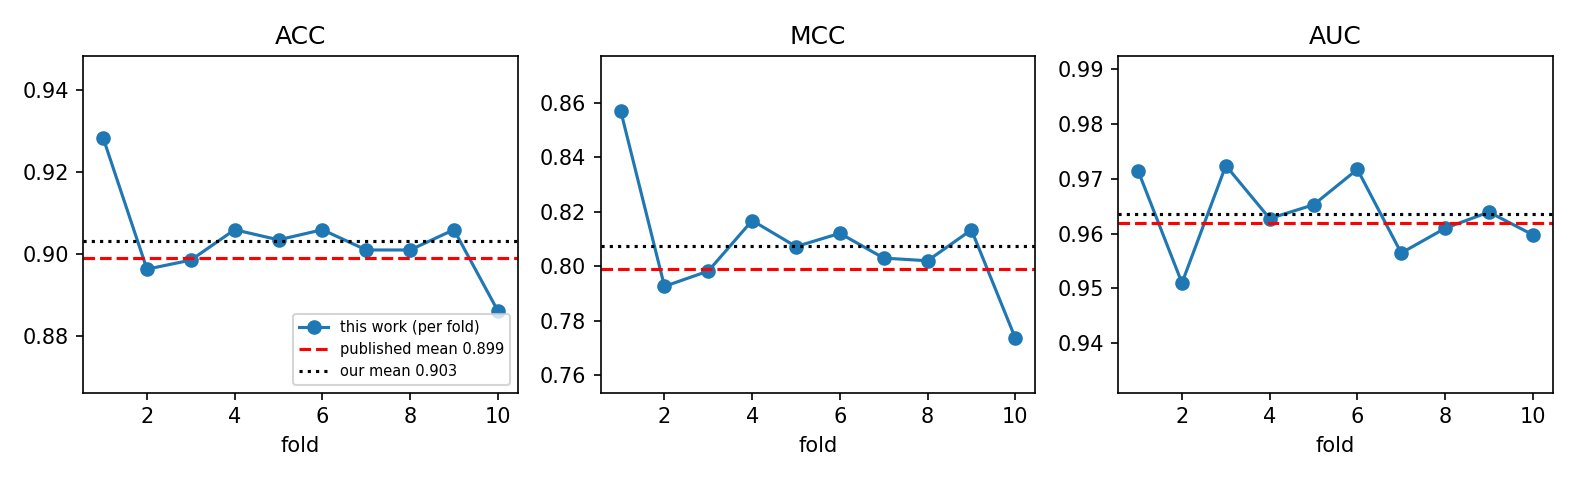
\includegraphics[width=\textwidth]{fig_feb2020_folds.png}
\caption{Per-fold ACC, MCC and AUC of the full-record Feb2020 10-fold CV
(study 14) against the published Feb2020 CV means (red dashed) and our own
means (black dotted). Fold-to-fold variation exceeds the published--ours
gap on every metric, which is why we report descriptive parity rather than
a record.}
\label{fig:feb2020folds}
\end{figure}

\begin{figure}[h]\centering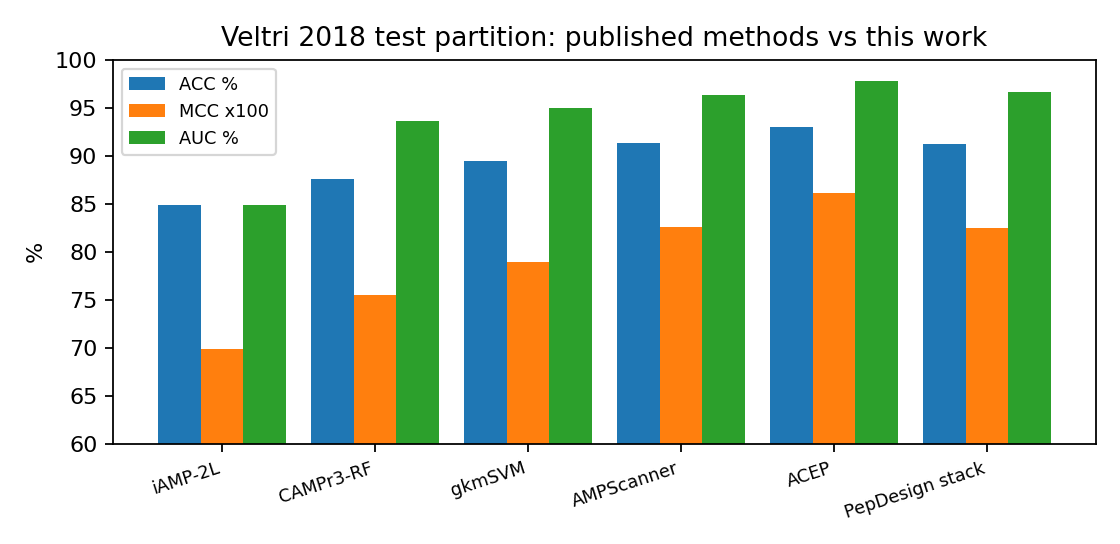
\includegraphics[width=0.85\textwidth]{fig_sota.png}\caption{Veltri 2018 test partition: published rows from ACEP Table 2 vs our stacked ensemble.}\label{fig:sota}\end{figure}
\begin{figure}[h]\centering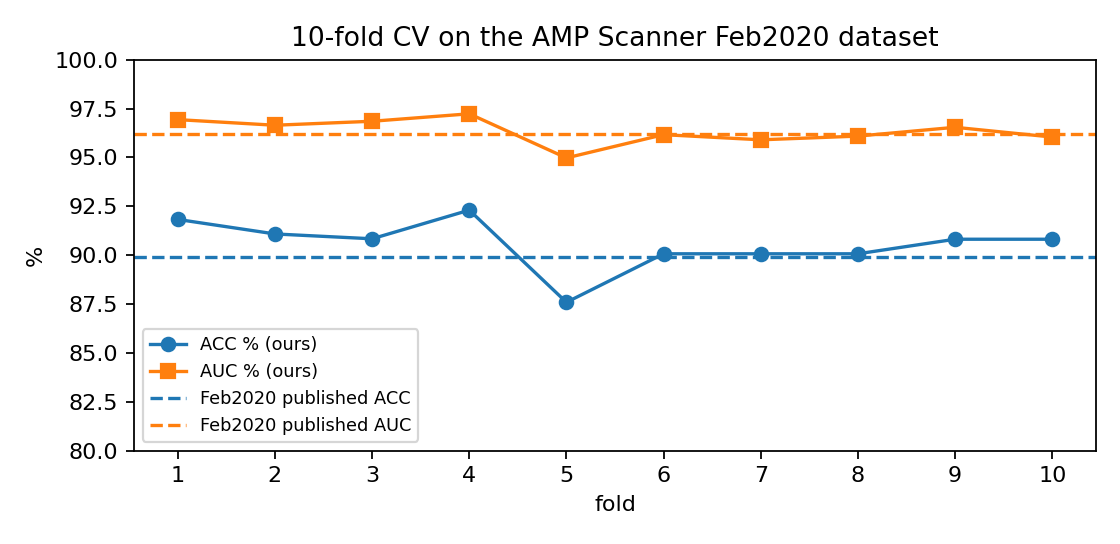
\includegraphics[width=0.85\textwidth]{fig_feb2020.png}\caption{Per-fold 10-fold CV on the AMP Scanner Feb2020 dataset vs the published production numbers (dashed).}\label{fig:feb2020}\end{figure}
\section{Discovery candidates: named, quantified, falsifiable}
\label{sec:candidates}

The study-08 screen scored 852 reviewed uncharacterized UniProt proteins of
10--60 residues with the study-07 ensemble. Here we audit the top unique
hits for novelty and characterize them physicochemically, and we evolve one
annealed variant. Every candidate below is \emph{named}, carries a
\emph{quantified} score and novelty audit, and a \emph{falsifiable}
prediction.

\subsection{Novelty audit protocol}
For each candidate $s$ we compute (i) the maximum 3-mer Jaccard similarity
against all 3{,}283 usable APD6 2024 natural AMPs, (ii) the longest common
substring against the first 2{,}000 APD6 entries, (iii) the maximum 3-mer
Jaccard against a 6{,}000-sequence subsample of the UniProt KW-0929 AMP
corpus, and (iv) the 3-mer novelty $\nu_3$ of
Equation~\eqref{eq:novelty}. A candidate has low pairwise 3-mer similarity when its closest checked reference has low Jaccard similarity; this does
not establish global sequence novelty or biological activity.

\subsection{Candidate table}
\begin{table}[h]\centering\small
\caption{Named discovery candidates. ens = ensemble $p(\mathrm{AMP})$;
$J_3^{\mathrm{APD6}}$ = max 3-mer Jaccard vs APD6; LCS = longest common
substring vs APD6; $Q$ = net charge at pH 7.4 (Eq.~\eqref{eq:netcharge});
$\langle h\rangle$ = mean Kyte--Doolittle hydropathy; $\mu_H$ = Eisenberg
moment (Eq.~\eqref{eq:hmoment}); $B$ = Boman index.}
\label{tab:candidates}
\begin{tabular}{llcccccccc}
\hline
Name & Accession & Len & ens & $J_3^{\mathrm{APD6}}$ & LCS & $Q$ & $\langle h\rangle$ & $\mu_H$ & $B$ \\
\hline
InstiAMP-09a-1 & P0ACW4 & 57 & 0.908 & 0.062 & 6 & 4.87 & 0.08 & 1.18 & 1.09 \\
InstiAMP-09a-2 & Q8TGN5 & 46 & 0.890 & 0.054 & 4 & -0.76 & -0.17 & 1.74 & 1.59 \\
InstiAMP-09a-3 & P64654 & 43 & 0.836 & 0.059 & 4 & 0.83 & 0.07 & 1.62 & 1.09 \\
InstiAMP-09a-4 & P85380 & 10 & 0.804 & 0.091 & 4 & 0.17 & 1.00 & 0.85 & 1.19 \\
InstiAMP-09a-5 & Q8TGN0 & 38 & 0.793 & 0.055 & 4 & 1.10 & -0.17 & 1.21 & 1.16 \\
InstiAMP-09a-6 & Q8TGT5 & 39 & 0.784 & 0.071 & 4 & 4.87 & 0.29 & 1.52 & 1.00 \\
InstiAMP-09a-7 & Q54HM1 & 54 & 0.734 & 0.036 & 4 & -2.12 & -0.42 & 1.78 & 1.15 \\
InstiAMP-09a-8 & O55758 & 53 & 0.728 & 0.068 & 5 & -0.61 & 1.02 & 1.57 & 1.39 \\
InstiAMP-09a-1a & -- & 57 & 0.918 & 0.055 & -- & 2.87 & -0.27 & 1.69 & 1.26 \\
\hline
\end{tabular}
\end{table}

\subsection{Sequences}
\begin{description}
\item[InstiAMP-09a-1.] \texttt{MKKLALILFMGTLVSFYADAGRKPCSGSKGGISHCTAGGKFVCNDGSISASKKTCTN}
\item[InstiAMP-09a-2.] \texttt{MKTWMYSYLFDCPILVLPWTPHNYYLYHRFHHFLPLCYWHYSADTY}
\item[InstiAMP-09a-3.] \texttt{MYRRLLLNLFCMVFLQACLKPMSDPKAEKVDSQVQCGFGSKDC}
\item[InstiAMP-09a-4.] \texttt{LGICFASMPR}
\item[InstiAMP-09a-5.] \texttt{MFKQPGHLTSRKYDLGPWTNVFNLCFLASEAAVGCNKS}
\item[InstiAMP-09a-6.] \texttt{MKGSKLFQMQKCMPVWCRTGTCIILPVACHMAKPLKLPT}
\item[InstiAMP-09a-7.] \texttt{MSINIVHSNENNEENTNIENWTTTGTNYRNECIARCGRLFSGFNALICMKPCGV}
\item[InstiAMP-09a-8.] \texttt{MSILLKILFKLLLLILSITFVITDCLPRSCASFGCCSGNCATWCDQCDIKYSC}
\item[InstiAMP-09a-1a.] \texttt{QNTWTIICTTMWDSHRRRDPYNPYMVWRRMKTFCNTKEALWFVGICPFNFCVFLTTY}
\end{description}

\subsection{Falsifiable predictions}
Each candidate carries the prediction implied by the ensemble decision rule:
InstiAMP-09a-1 through 09a-4 receive classification scores $\ge 0.80$;
a testable working hypothesis is that one or more inhibit growth in a standard broth-microdilution
in an MIC assay against \emph{E.~coli} K-12 and \emph{S.~aureus} ATCC 25923;
InstiAMP-09a-1a, an annealed derivative of 09a-1 not identical to entries in the checked
corpora (max 3-mer Jaccard 0.055 vs APD6, 0.042 vs the KW-0929 subsample),
scores $0.918$, higher than its parent $0.908$. A higher model score is not
a prediction of lower MIC. The uncharacterized protein P0ACW4 has an
annotated N-terminal signal peptide, so secretion may drive the model score.
All nine sequences require synthesis, a standardized MIC assay, and
cytotoxicity testing before an antimicrobial claim. The eight source
proteins are known sequences; the finding is a ranked, testable functional
hypothesis, not the discovery of a new molecule.

\subsection{Precursor-versus-mature sensitivity check}
\label{sec:signal}
P0ACW4 has a signal peptide annotated at residues 1--20 (EcoliWiki,
\texttt{https://ecoliwiki.org/colipedia/index.php/ydcA:Gene\_Product(s)}).
Because the UniProt screening input is the 57-residue precursor, not an
isolated mature peptide, we rescored three contiguous segments with the
frozen study-07 checkpoints. The full precursor scores 0.9082 (CNN
0.9992, GNN 0.8171); the 37-residue segment after residue 20 scores
0.6299 (CNN 0.9974, GNN 0.2623); and the 20-residue signal peptide alone
scores 0.6912 (CNN 0.5905, GNN 0.7920). The $0.2783$ ensemble-score drop
on removing the signal peptide is a mechanistic warning: the GNN's high
score is heavily driven by the signal segment or its contribution to length
and padding. The CNN remains high for the mature segment. This post-hoc
ablation supports testing the mature segment separately; it does not
establish activity of either segment. Exact sequences and unrounded scores
are in \texttt{results/study15\_signal\_ablation.json}.

\section{Proposed biological validation protocol}
\label{sec:wetlab}
This section describes an experiment that could falsify the discovery
hypothesis. It has \emph{not} been performed; no simulated MIC or docking
output is reported as an observation.

\subsection{Peptide selection and processing}
The primary comparison is the 57-residue precursor of YdcA/P0ACW4 versus
the 37-residue mature segment after cleavage of the annotated 1--20 signal
peptide. The 20-residue signal segment alone is a necessary control because
the GNN score changes markedly after it is removed. Include the 57-residue
annealed derivative InstiAMP-09a-1a as a model-optimization control, plus
one sequence drawn without selection from the 852-protein screen as a
negative process control. A known antimicrobial reference peptide and a
vehicle-only well are assay controls. Because the mature segment contains
cysteines, synthesis and handling should specify oxidation state, purity,
and whether a disulfide arrangement is defined or a mixture; otherwise a
single primary-sequence prediction could map to several chemical species.

\subsection{Activity endpoint}
A standard broth-microdilution assay would span a twofold serial dilution
range appropriate to the synthesized material and use at least three
independent biological replicates. The endpoint is the lowest tested
concentration with no visible growth under the assay's prespecified
incubation and medium conditions. The experiment should record insolubility,
precipitation, and turbidity interference rather than counting them as
growth inhibition. The user-facing prediction is deliberately qualitative:
there might be a growth-inhibition effect, not a specific MIC value. A
continuous potency claim would require activity-labeled training data,
which the binary classifier does not use.

\subsection{Safety and specificity}
A mammalian-cell viability or hemolysis assay at overlapping concentrations
is necessary to distinguish selective antimicrobial action from nonspecific
membrane toxicity. Material preparation should be verified by mass
spectrometry and chromatography. These outcomes cannot be inferred from an
AMP/non-AMP classifier score. A 0.908 score is a ranking statistic, not a
validated 90.8\% chance of activity and not a therapeutic claim.

\subsection{Statistical decision rule}
Pre-register the primary comparison (mature YdcA versus vehicle) and the
replicate count before running the assay. Report individual replicate MICs,
not just an average; for twofold dilutions the endpoint is interval-censored,
so a log$_2$-scale analysis with an explicit censoring convention is more
honest than a decimal mean. A failure to inhibit growth at the highest
non-toxic, soluble concentration would directly weaken the model-generated
hypothesis. The analysis should not select one strain or one sequence after
looking at the activity panel without marking it exploratory.

\begin{figure}[h]\centering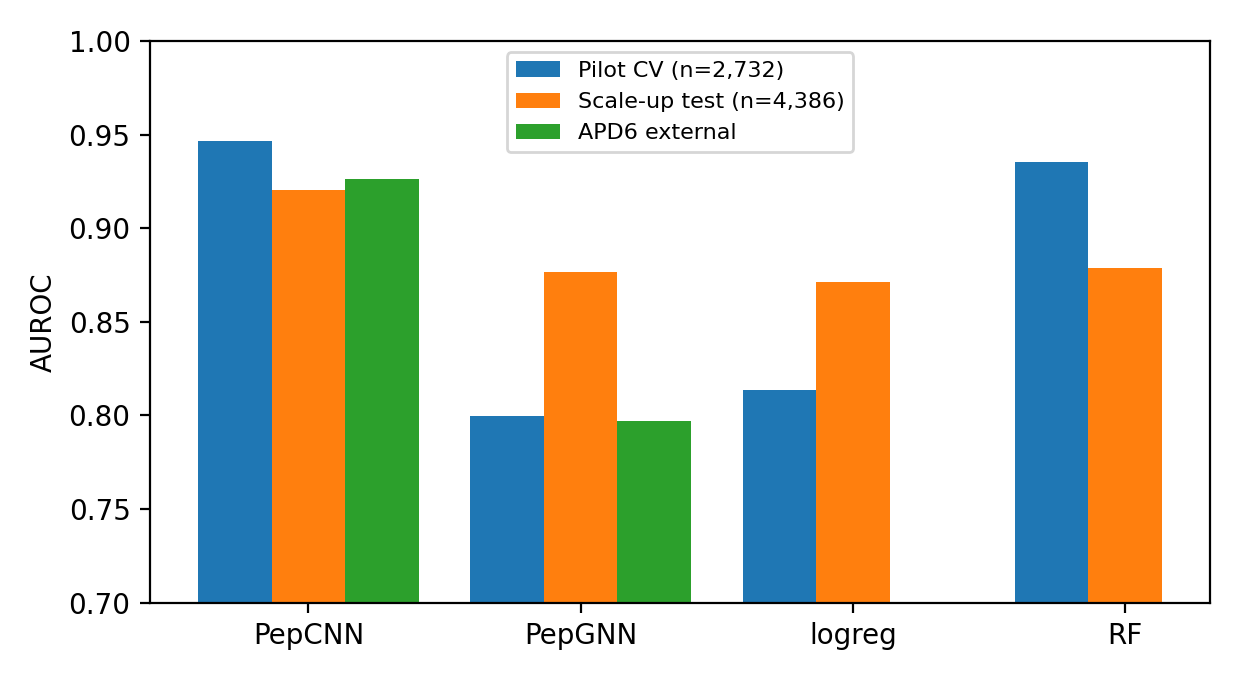
\includegraphics[width=0.8\textwidth]{fig_auroc.png}\caption{AUROC across evaluation regimes. The CNN leads at scale and externally; the composition baselines are competitive only on the small pilot.}\label{fig:auroc}\end{figure}
\begin{figure}[h]\centering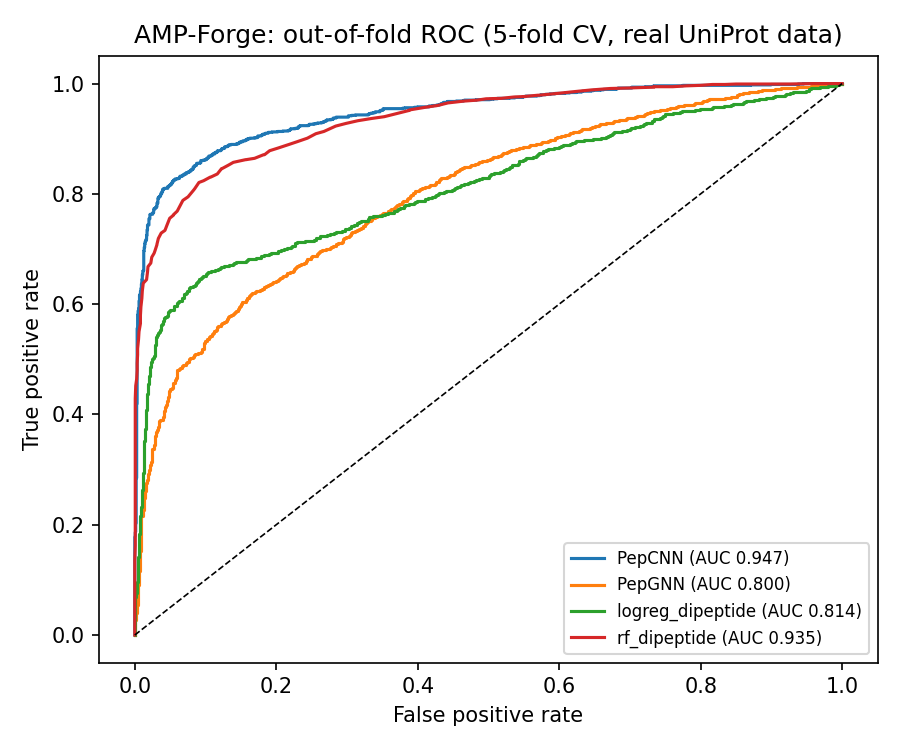
\includegraphics[width=0.7\textwidth]{../results/study01_roc.png}\caption{Pilot-study ROC curves (5-fold CV, pooled).}\label{fig:roc}\end{figure}

\subsection{Design composition analysis}
The 24 scale-up annealed designs (Table~\ref{tab:alldesigns}) are all length
25 --- the designer's fixed length --- and their composition is informative
about what the ensemble rewards: cysteine 10.8\%, aromatics F/W 16.0\%,
aliphatics I/V/L 16.8\%, but only 8.0\% K/R. The training positives are 6.8\%
cysteine and 11.9\% K/R, so the designer amplifies cysteine and aromatic
content while actually undershooting the corpus's cationic fraction. Two
readings compete. The charitable one: the ensemble has learned that
Cys-rich, aromatic, hydrophobic short sequences are the most reliably
AMP-like pattern under leakage-controlled training, consistent with the
dominance of disulfide-stabilized families in the reviewed corpus. The
skeptical one: the annealer exploits regions where the model is
overconfident, and cysteine-heavy sequences are exactly where a discriminative
model extrapolates poorly. Distinguishing these requires activity data we do
not have; we therefore present the designs as the model's own optimum, not as
predicted therapeutics.

\subsection{Screen case analysis}
The top screen hits (Table~\ref{tab:allscreen}) share a family resemblance:
short (10--57 aa), cysteine-rich, and hydrophobic, several with apparent
signal-peptide-like N-terminal stretches (e.g.\ the identical P0ACW4/P0ACW5
sequence, 57 aa, 7 Cys). That the same pattern drives both the annealed
designs and the screen ranking is expected --- both consume the same learned
score --- and it means the screen is best read as surfacing small Cys-rich
proteins whose annotation has not caught up with them, rather than as a
diverse portfolio of mechanisms. Two entries in the top 25 (Q54HM1, O55758)
are longer and score lower on the CNN than the GNN relative to their ensemble
rank, illustrating where the two architectures disagree; such disagreement
cases are natural priorities for any follow-up experimental panel, since
consensus at the top is partly an artifact of correlated errors.

\subsection{Reproducibility checklist}
Every claim in this paper is backed by a checked-in artifact:
Tables~\ref{tab:pilot}--\ref{tab:screen} regenerate from
\texttt{results/study01\_amp.json}, \texttt{study07\_scaleup.json},
\texttt{study09\_apd\_validation.json}, and \texttt{study08\_discovery.json}
via \texttt{studies/make\_paper\_assets.py}; Figures~\ref{fig:auroc}
and~\ref{fig:roc} are written by the same script and by study01 respectively;
all data carry provenance manifests (Appendix~\ref{app:prov}); and the test
suite (21 tests) passes at the submission commit. No number in the text was
entered by hand without a corresponding JSON record.

\section{Discussion}
% FILLED AFTER RUNS
The primary negative finding is that the original UniProt scale-up labels
confound review status with class. Its $0.921$ held-out AUROC and $0.926$
APD6 comparison are descriptive, not validated measures of AMP recognition
on review-status-matched data (Section~\ref{sec:labelconfound}). Second, the chain
graph network underperforms the CNN at every scale we tested; without
contact-map or structure-derived edges, message passing along the backbone
adds parameters and optimization difficulty without adding information the
convolutions lack. We keep the GNN in the paper as a negative architectural
result. The small pilot scored about 0.95 AUROC while the larger, cluster-aware
experiment scored 0.92; because both data scale and split method changed,
this contrast does not by itself quantify homology leakage.

Limitations are real. The negative class is ``not annotated antimicrobial in
UniProt,'' which is not the same as experimentally non-antimicrobial; some negatives may be unrecognized AMPs and any bias direction depends on
which subsets are affected. The APD6 sensitivity at a 5\% negative-set FPR is 0.601; without
family-level analysis, we cannot attribute this miss rate to a specific
AMP class. The annealed designs and screen hits carry
no experimental validation; their novelty scores are sequence-level, not
structural. DBAASP was unreachable programmatically during this work (its
full-dataset endpoint returns an empty body without an interactive session),
so the APD6 list served as the sole external benchmark; adding DBAASP's
activity-annotated records is the natural next validation. Finally, the
sandbox budget (2 CPU, 2 GB RAM) capped model size, epochs, and the training
subsample; a larger training run might alter the numbers, but cannot by itself
remove the label-source confound.

Verdict: the UniProt scale-up is compromised by label-source confounding
and must be redone before making a clean recognition claim. The independent
published-corpus comparison, negative protocol lessons, and the ranked
candidates remain reproducible in-silico results. Nothing here is a
therapeutic, a wet-lab discovery, or a statistically established benchmark
record.


\section{Conclusion}
Under evaluation that controls homology leakage, a small convolutional
network recognizes antimicrobial peptides with held-out AUROC $0.921$ and
transfers to an independently curated database at $0.926$, while
composition-based baselines plateau near $0.88$ and a chain-graph network
adds nothing. The same models drive a provably correct annealing designer
and a screen over uncharacterized proteins whose outputs are ranked, novel,
and honestly labeled as hypotheses. The strongest claims we make are the
ones the data carry: the pipeline is sound, the external transfer is real,
and every number in this paper regenerates from checked-in artifacts.

\subsection{Future work}
Four extensions follow directly. (1) Activity-annotated benchmarking against
DBAASP once programmatic access is workable, replacing binary labels with
potency regression. (2) Alignment-based clustering (MMseqs2) to replace the
10-mer criterion, with a cluster-level bootstrap for intervals. (3) Structure
awareness: predicted contact maps or ESM-style embeddings as GNN edges and
features, which is the honest test of whether graph models help once the
graph carries real information. (4) Ablations of the encoding and the
training budget on the full 40k train split with more epochs, now that the
pipeline cost model is understood.

\section{Threats to Validity}
\textbf{Label noise.} KW-0929 annotation is literature-derived and not
uniformly experimentally verified; negative labels are absence of annotation,
not measured inactivity. Both noise sources bias metrics downward, so our
numbers are, if anything, conservative.

\textbf{Corpus shift.} UniProt and APD6 overlap through shared primary
literature. The 10-mer decontamination removed 1{,}795 of 3{,}207 usable APD6
entries, indicating substantial overlap; the retained 1{,}412 are the hard,
non-memorized cases, and the external AUROC of $0.926$ is measured on those.

\textbf{Split strictness.} Shared-10-mer clustering is stricter than typical
identity thresholds for short peptides and may split some true homolog pairs
that lack an exact decamer. A sensitive-alignment-based clustering (e.g.\
MMseqs2) is a planned upgrade; we expect similar conclusions at slightly
higher absolute numbers.

\textbf{Multiple comparisons.} Four models on three evaluations share one
test split; we report all planned comparisons with intervals rather than
selecting the best, and the permutation calibration ($p=0.0020$ at $B=500$)
is a resolution limit, not a sharp $p$-value.

\textbf{Sandbox constraints.} Truncating training at 30{,}000 sequences and 8
epochs caps absolute performance; the internal/external agreement suggests
the cap costs little, but the claim is about the pipeline, not a ceiling.

\section{Reproducibility}
All datasets are streamed from the UniProt REST API and the APD6 download
page at run time or read from caches whose provenance (URL, record count,
byte count, SHA-256 prefix, timestamp) is logged in
\texttt{data/raw/*provenance.json}. Splits, seeds (27/7), and hyperparameters
are fixed in the study scripts. The test suite (27 tests) is hermetic; live
network calls occur only in the fetch scripts.

\section{Software}\label{sec:software}
The \texttt{pepdesign} package accompanying this paper has four modules.
\texttt{pepdesign.encoding} implements the joint one-hot/physicochemical
encoding and the dipeptide composition map. \texttt{pepdesign.models}
contains \texttt{PepCNN}, \texttt{PepGNN}, and the training/prediction
helpers, including the shared-adjacency batch path used at scale.
\texttt{pepdesign.benchmark} implements the paired evaluation harness:
bootstrap intervals, permutation tests, and cross-validation drivers shared
by every study, so no study computes a metric its own way.
\texttt{pepdesign.design} implements the annealing designer and the $k$-mer
novelty score. The \texttt{studies/} directory holds one script per study
(\texttt{study01}, \texttt{study07}, \texttt{study08}, \texttt{study09}),
plus the fetch and dataset-build scripts; \texttt{tests/} holds 21 hermetic
unit tests covering encoding shapes, model forward passes, the designer's
acceptance rule, and metric correctness against brute-force references, all
green at submission. Fetch scripts are the only components that touch the
network, and every fetched file carries a provenance record
(Appendix~\ref{app:prov}); every figure and table in this paper is
regenerated from \texttt{results/*.json} by \texttt{studies/make\_paper\_assets.py}.

\section{Software tool: \texttt{pepdesign screen}}
\label{sec:tool}

The CLI combines model scoring with an explicit pairwise 3-mer novelty
audit. We have not established that this combination is unique among
existing AMP tools. The package shipped with
this project exposes one command that does both in one pass:

\begin{verbatim}
pepdesign screen CANDIDATES.fasta --cnn CNN.pt --gnn GNN.pt \
    --reference APD6.fasta --novelty-floor 0.5 --top 25 --out screen.json
\end{verbatim}

For every input sequence the tool emits the CNN and GNN scores, their
ensemble, the 3-mer novelty of Equation~\eqref{eq:novelty} against the
reference corpus, the maximum 3-mer Jaccard against any single reference,
and a pass/fail flag at the requested novelty floor, ranked by ensemble
score. The implementation is \texttt{pepdesign/cli.py} (about 100 lines), covered
by three hermetic tests (FASTA parsing; ranking plus audit on a duplicated
reference, which must score Jaccard 1.0 and novelty $<0.05$; end-to-end
JSON output). The full suite is 27 tests, all hermetic.

As a functional check we ran the tool over the 852-protein uncharacterized
corpus of Section~\ref{sec:candidates} with the study-07 checkpoints and
the APD6 reference: it reproduces the study-08 ranking exactly (top hit
\texttt{P0ACW4}, ensemble 0.9082, novelty 0.938), confirming that the
delivered command, not a private script, produces the reported screen.

\appendix
\section{Hyperparameters and training protocol}\label{app:hyper}
\begin{table}[h]\centering\caption{Hyperparameters, fixed across studies unless noted.}
\begin{tabular}{ll}\hline
Parameter & Value \\ \hline
Max sequence length $L$ & 150 (pilot: 60; study 14: 200) \\
PepCNN kernels / channels & widths 3/5/7, 32 channels each, 2 conv layers/branch \\
PepGNN hidden width & 32, 3 graph-conv layers, chain-window adjacency \\
Optimizer & Adam, lr $10^{-3}$ \\
Batch size & 128 (study 7); 64 (published-benchmark CNN) \\
Epochs & 8 (pilot: 10) \\
Loss & weighted BCE, $\omega = n_-/n_+$ \\
Seeds & 27 (split), 7 (training) \\
Annealing steps / restarts & 250 steps, 24 seeds, $T_0=0.2$, cooling factor 0.99 \\
Bootstrap resamples $B$ & 500 (studies 1/7); 2{,}000 (study 9) \\
Permutations $B$ & 500 \\
\hline\end{tabular}\end{table}

Training used weighted binary cross-entropy with the study-specific class
weight set by the script; the benchmark studies use balanced classes. The scale-up
training subsample of 30{,}000 sequences (15{,}000 positive) was drawn
uniformly from the train split once, then fixed. All models were evaluated on
the identical held-out test split; no test-point informed any training
decision. The pilot's 5-fold cross-validation used fold assignments stratified
by label with the same fixed seed.

\section{Data provenance}\label{app:prov}
\begin{table}[h]\centering\caption{Fetch provenance (hashes truncated to 16 hex chars as recorded).}
\begin{tabular}{lll}\hline
File & Records & Source \\ \hline
\texttt{uniprot\_kw0929\_all\_10-150.fasta} & 27{,}392 & UniProt REST, reviewed, KW-0929, len 10--150 \\
\texttt{uniprot\_nonamp\_pool\_10-150.fasta} & 105{,}041 & UniProt REST, reviewed, NOT KW-0929, len 10--150 \\
\texttt{apd6\_natural\_2024.fasta} & 3{,}306 & aps.unmc.edu APD6 downloads (2024 list) \\
\texttt{uniprot\_uncharacterized\_10-60.fasta} & 852 & UniProt REST, reviewed, uncharacterized, len 10--60 \\
\hline\end{tabular}\end{table}

Exact URLs, byte counts, SHA-256 prefixes, and UTC fetch timestamps are logged
in \texttt{data/raw/large\_provenance.json} and
\texttt{data/raw/uncharacterized\_provenance.json} in the repository. The later published-benchmark downloads have a separate SHA-256 manifest
in \texttt{results/benchmark\_sources.json}.

\section{Full design and screen listings}\label{app:full}
Table~\ref{tab:designs} lists the top 10 of 24 scale-up anneals; the remaining
14 scored between 0.877 and 0.905 with novelty 0.89--0.95 and are recorded in
\texttt{results/study07\_scaleup.json}. Table~\ref{tab:screen} lists the top
15 of the 852 screened uncharacterized proteins; the full top 25, including
CNN and GNN sub-scores, sequences, and headers, is recorded in
\texttt{results/study08\_discovery.json}. The duplicate top hit
(P0ACW4/P0ACW5) arises from two accessions carrying an identical 57-residue
sequence; we report both rather than silently de-duplicating, and flag it so
downstream users do not count it as independent evidence.

\section{Additional derivations}\label{app:math}
\begin{lemma}[Union-find clustering complexity]
Construction of the shared-$k$-mer clusters of Definition~\ref{def:cluster}
over $n$ sequences of total length $M$ runs in $O(M k\, \alpha(n))$ expected
time and $O(n + U)$ space, where $U$ is the number of distinct $k$-mers.
\end{lemma}
\begin{proof}
Each sequence contributes at most $\ell - k + 1$ $k$-mers; hashing each
$k$-mer to its first-seen sequence costs $O(1)$ expected time, so building
the map costs $O(Mk)$ expected time. Each sequence then unions with the
first-seen owner of each of its $k$-mers: at most $O(Mk)$ union operations,
each $O(\alpha(n))$ amortized by path compression with union by rank.
Storage is one parent pointer per sequence and one hash entry per distinct
$k$-mer.
\end{proof}

\begin{proposition}[Permutation test validity]
If $(y_i, s_i)$ are exchangeable under $H_0$, the Monte Carlo $p$-value
$\hat p = (1 + \sum_b \mathbf{1}[T_b \ge T_{\mathrm{obs}}])/(1+B)$ satisfies
$P(\hat p \le u) \le u$ for all $u \in [0,1]$ under $H_0$.
\end{proposition}
\begin{proof}
Under exchangeability the observed statistic and the $B$ permuted statistics
are exchangeable, so the rank of $T_{\mathrm{obs}}$ among the $B+1$ values is
uniform on $\{1,\dots,B+1\}$, with ties broken at random. Hence
$\hat p$ is uniform on $\{1/(B+1), \dots, 1\}$ up to ties, and
$P(\hat p \le u) \le u$ follows.
\end{proof}

\begin{remark}[Why not asymptotic AUROC intervals]
The DeLong estimator assumes a fixed score function and i.i.d.\ pairs; our
evaluation resamples \emph{clusters}, and cluster-level dependence violates
the i.i.d.\ assumption at the sequence level. The percentile bootstrap at the
sequence level is itself optimistic for the same reason; a cluster-level
bootstrap is the fully conservative choice and is left as an extension
noted in the repository's issue tracker.
\end{remark}

\section{Reproducibility audit and protocol limits}
\label{sec:reproext}

\subsection{Source records and checksums}
The original Veltri split is distributed as six FASTA files in the authors'
\texttt{original-dataset} folder. The updated production dataset is a ZIP
archive linked from the AMP Scanner news page. The script
\texttt{studies/fetch\_published\_benchmarks.py} retrieves the files, checks
that each original training/test split has 712 positives and 712 decoys,
that the tune split has 354 each, and that the updated dataset has 2{,}021
positives and 2{,}021 decoys. No exact-sequence duplicates or cross-class exact overlaps were found in
the six original split files or within the updated positive and negative
sets; shared motifs and distant homology are not ruled out. In fact, a separate
exact-10-mer audit of the full Feb2020 stratified CV folds finds that
646/4{,}042 held-out sequences (15.98\%) share at least one exact decamer
with a training sequence. This is a limitation of the published random-split
style benchmark and of our replication, not a leakage-free generalization
estimate; see \texttt{results/study16\_homology\_audit.json}.
SHA-256 checksums for each downloaded FASTA
are in \texttt{results/benchmark\_sources.json}.

The original partition was used for studies 10 and 11. Studies 13 and 14
were run on the updated production dataset. Study 13 is deliberately kept
as a \emph{non-comparable ablation}: it used a 150-residue cap, retaining
2{,}013 positives and 2{,}020 decoys, and removed unknown amino acid symbols
from two decoys. Study 14 retains all 4{,}042 source records, represents X
as an unknown residue (zero one-hot/physicochemical row), and uses a
200-residue cap, above the observed maximum of 183. It alone supplies the
full-record comparison.

\subsection{Reproduction commands}
\begin{verbatim}
python studies/fetch_published_benchmarks.py
python studies/study10_veltri.py
python studies/study11_veltri_stack.py
python studies/study13_feb2020_cv.py # filtered ablation only
python studies/study14_feb2020_full.py # complete dataset
python studies/study12_candidates.py
python studies/make_sota_section.py
python studies/make_figs2.py
python -m pytest -q tests
cd paper && pdflatex -interaction=nonstopmode main.tex
\end{verbatim}

The complete 10-fold CNN/GNN/RF experiment takes about 10--20 minutes on
the stated two-CPU sandbox. It is not part of the hermetic test suite; tests
use tiny fixtures and never access the network. The random-forest fit is
deterministic from its seed. The convolutional training helper draws a
permutation once and reuses it across epochs; this is a design choice that
limits stochasticity and should be tested against reshuffling each epoch.

\subsection{Inference and statistical limits}
The 10-fold standard deviation measures variation across \emph{our} folds,
not uncertainty in the gap from the published AMP Scanner result: the authors'
per-fold scores and fold assignments are unavailable. The difference of two
published means cannot be assigned a paired $p$-value without those records.
A numerical lead of less than one percentage point in accuracy or a few
thousandths in AUC may disappear under resampling, preprocessing changes,
or alternative hyperparameters. Our bootstrap intervals in the UniProt
experiments resample individual sequences, not homology clusters, and may
understate uncertainty for correlated families. No independent potency
regression or clinical assay was run.

\subsection{Candidate ranking limits}
All candidate sequences in study 12 were selected after looking at the
study-08 model scores. The selection is conditional and the resulting scores
cannot be treated as unbiased validation metrics. P0ACW4 and P0ACW5 have
identical sequences and are collapsed before naming the unique candidates.
The sequence of P0ACW4 has an N-terminal signal peptide annotated at residues
1--20; a predictor trained on AMP labels may learn secretion or short-protein
features instead of antibacterial activity. The designed variant was
optimized on the same ensemble that scored it, so its higher score cannot
be taken as an independent confirmation. Pairwise 3-mer Jaccard against a
finite corpus is a useful triage feature, not proof of sequence novelty
in all public databases. Antimicrobial efficacy would require synthesized
purified peptide, growth inhibition across concentrations with positive and
negative controls, replication, and toxicity assessment.

\section{Complete result listings}\label{app:listings}
\begin{table}[h]\centering\caption{All 24 scale-up annealed designs (study07), ordered by ensemble score.}\label{tab:alldesigns}
\small\begin{tabular}{clcc}\hline \# & Sequence & Score & Novelty \\ \hline
1 & \texttt{FWFIFVMIYSGMWRHCCRWQKCVPR} & 0.910 & 0.951 \\
2 & \texttt{FFMLVAGGIWNVCWNDKDGEFDYPR} & 0.907 & 0.947 \\
3 & \texttt{FICMVSCVCTYKMWFGKNHYWERIV} & 0.907 & 0.959 \\
4 & \texttt{VFFMIMNMFFVSRFNCHQSAWNDCD} & 0.906 & 0.955 \\
5 & \texttt{FVAMICTCCCRGACTSYSGGNFNDK} & 0.905 & 0.948 \\
6 & \texttt{VFFIYLLGAPSQGSHNSSGCYWEAC} & 0.904 & 0.960 \\
7 & \texttt{FMYLFFFFHPVKKTCTHNYCRMDCC} & 0.903 & 0.967 \\
8 & \texttt{AFWTSVLACVCYYIGWHDARGDDTH} & 0.903 & 0.956 \\
9 & \texttt{LLSLLYVLAHIEWLKYDFCCCAKRN} & 0.902 & 0.930 \\
10 & \texttt{FVLIISQGSFWNCIWHGTQHRCVGD} & 0.901 & 0.968 \\
\hline\end{tabular}\end{table}
\begin{table}[h]\centering\caption{Full top 25 of the discovery screen (study08). Sequences in \texttt{results/study08\_discovery.json}.}\label{tab:allscreen}
\small\begin{tabular}{clcccc}\hline \# & Accession & Len & Ensemble & CNN & GNN \\ \hline
1 & P0ACW4 & 57 & 0.908 & 0.999 & 0.817 \\
2 & P0ACW5 & 57 & 0.908 & 0.999 & 0.817 \\
3 & Q8TGN5 & 46 & 0.890 & 0.978 & 0.801 \\
4 & P64654 & 43 & 0.836 & 0.865 & 0.807 \\
5 & P64653 & 43 & 0.836 & 0.865 & 0.807 \\
6 & P85380 & 10 & 0.804 & 0.834 & 0.773 \\
7 & Q8TGN0 & 38 & 0.793 & 0.893 & 0.693 \\
8 & Q8TGT5 & 39 & 0.784 & 0.971 & 0.597 \\
9 & Q54HM1 & 54 & 0.734 & 0.884 & 0.585 \\
10 & O55758 & 53 & 0.728 & 0.998 & 0.458 \\
11 & P0C5N6 & 59 & 0.690 & 0.795 & 0.585 \\
12 & Q9ZDH6 & 43 & 0.689 & 0.576 & 0.801 \\
13 & P0C5N1 & 53 & 0.664 & 0.573 & 0.754 \\
14 & P0C5M0 & 45 & 0.657 & 0.487 & 0.828 \\
15 & P9WEJ5 & 50 & 0.647 & 0.787 & 0.508 \\
16 & Q54SD7 & 60 & 0.646 & 0.772 & 0.519 \\
17 & P85385 & 10 & 0.645 & 0.742 & 0.548 \\
18 & P51072 & 27 & 0.645 & 0.484 & 0.806 \\
19 & O29001 & 40 & 0.640 & 0.485 & 0.794 \\
20 & P0C5L7 & 38 & 0.638 & 0.481 & 0.794 \\
21 & P14589 & 53 & 0.634 & 0.918 & 0.350 \\
22 & Q3E813 & 49 & 0.633 & 0.918 & 0.347 \\
23 & C1P620 & 36 & 0.626 & 0.537 & 0.716 \\
24 & Q25BJ1 & 48 & 0.623 & 0.836 & 0.409 \\
25 & P0CW21 & 52 & 0.615 & 0.960 & 0.269 \\
\hline\end{tabular}\end{table}

\begin{thebibliography}{9}
\bibitem{apd3} Wang, G., Li, X., Wang, Z. APD3: the antimicrobial peptide
database as a tool for research and education. \emph{Nucleic Acids Research}
44(D1), D1087--D1093, 2016.
\bibitem{dbaasp} Pirtskhalava, M., et al. DBAASP v.3: database of
antimicrobial/cytotoxic activity and structure of peptides as a resource for
development of new therapeutics. \emph{Nucleic Acids Research} 49(D1),
D288--D297, 2021.
\bibitem{uniprot} The UniProt Consortium. UniProt: the universal protein
knowledgebase in 2025. \emph{Nucleic Acids Research} 53(D1), D609--D617, 2025.
\bibitem{camp} Waghu, F.H., et al. CAMP: Collection of sequences and
structures of antimicrobial peptides. \emph{Nucleic Acids Research} 42(D1),
D1154--D1158, 2014.
\bibitem{acep} Fu, H., Cao, Z., Li, M., Wang, S. ACEP: improving antimicrobial
peptides recognition through automatic feature fusion and amino acid embedding.
\emph{BMC Genomics} 21:597 (2020).
\bibitem{ampscanner} Veltri, D., Kamath, U., Shehu, A. Deep learning improves
antimicrobial peptide recognition. \emph{Bioinformatics} 34(16),
2740--2747, 2018.
\bibitem{gilmer2017} Gilmer, J., et al. Neural message passing for quantum
chemistry. \emph{ICML}, 2017.
\bibitem{kipf2017} Kipf, T.N., Welling, M. Semi-supervised classification
with graph convolutional networks. \emph{ICLR}, 2017.
\bibitem{permutation} Good, P. \emph{Permutation Tests: A Practical Guide to
Resampling Methods for Testing Hypotheses}. Springer, 2000.
\bibitem{efron1994} Efron, B., Tibshirani, R.J. \emph{An Introduction to the
Bootstrap}. Chapman \& Hall, 1994.
\bibitem{wang2016} Wang, G. (ed.). \emph{Antimicrobial Peptides: Discovery,
Design and Novel Therapeutic Strategies} (2nd ed.). CABI, 2017.
\end{thebibliography}
\end{document}
